\chapter{Themenkorb - Entwurfsmuster in der Datenmodellierung}
\section{History}
\begin{itemize}
    \item Um die Werte eines Attributs nachvollziehbar zu machen
    \item z.B. bei Preisen, Mitarbeitergehältern\dots
    \item Es gibt lückenlose \& lückenhafte Histories:
    \begin{itemize}
        \item lückenlos $\implies$ nur ein Datumswert(von / bis); muss teil des Primary-Keys sein
        \item lückenhaft $\implies$ zwei Datumswerte; einer muss teil des Primary-Keys sein
    \end{itemize}
\end{itemize}

\subsection{History eines Attributs}
\subsubsection{Allgemein}
\begin{itemize}
    \item z.B. um den Preis eines Produktes nachvollziehbar zu machen
    \item Es entsteht eine Extra-Entity mit folgenden Attributen (\textbf{PK})
    \begin{itemize}
        \item \textbf{Foreign Key auf die Ursprungsentity}
        \item \textbf{GueltigAb}
        \item Tatsächlicher Wert (gleicher Datentyp wie im Ausgangsmodell)
    \end{itemize}
\end{itemize}
\subsubsection{Abfragen}
\paragraph{Wert zu einem bestimmten Zeitpunkt bzw. aktueller Wert}
\begin{itemize}
    \item Um den aktuellen Preis zu bestimmen, muss die Datums-Klausel einfach "SYSDATE" enthalten.
\end{itemize}
\begin{figure}[H]
    \centering
    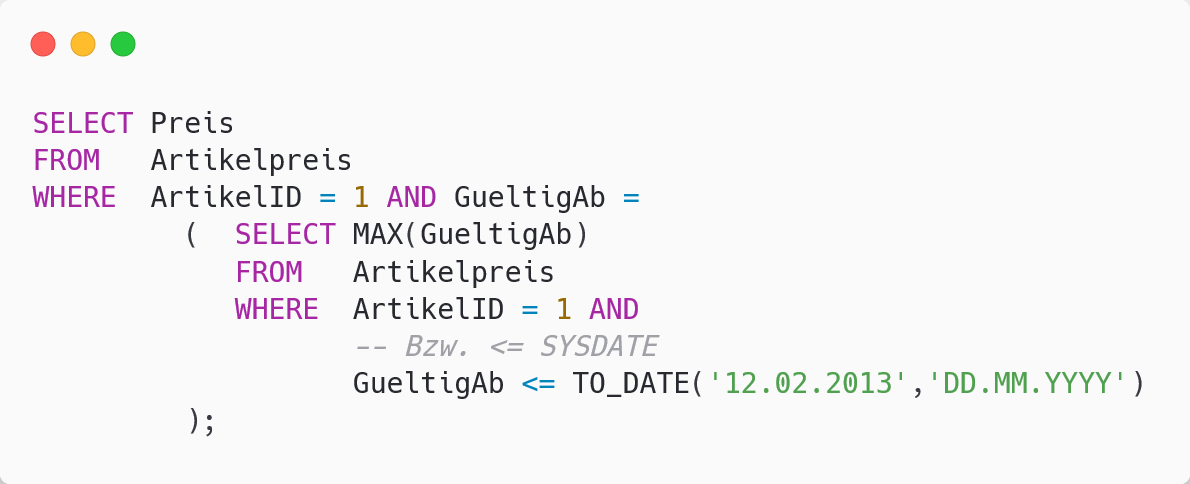
\includegraphics[width=\textwidth]{res/themenkorb_4/history_attribute.png}
\end{figure}

\subsection{History einer 1:n Beziehung}
\subsubsection{Allgemein}
\begin{itemize}
    \item z.B. um nachzuvollziehen, welcher Mitarbeiter wann in welcher Abteilung gearbeitet hat
    \item Es entsteht eine N:M Beziehung mit folgenden Attributen (\textbf{PK})
    \begin{itemize}
        \item Foreign-Key auf die fundamentale Entity
        \item \textbf{Foreign-Key auf die attributive Entity}
        \item \textbf{GueltigAb}
    \end{itemize}
\end{itemize}
\subsubsection{Abfragen}
\paragraph{Wert zu einem bestimmten Zeitpunkt bzw. aktueller Wert}
\begin{itemize}
    \item Um aktuelle Abteilung zu bestimmen, muss die Datums-Klausel einfach "SYSDATE" enthalten.
\end{itemize}
\begin{figure}[H]
    \centering
    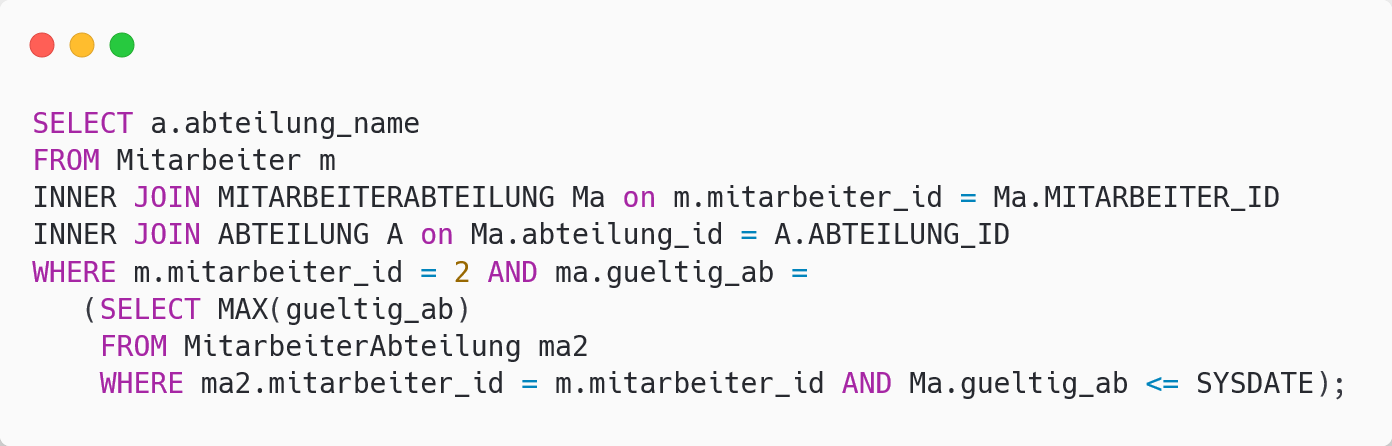
\includegraphics[width=\textwidth]{res/themenkorb_4/history_1_n.png}
\end{figure}

\subsection{History einer n:m Beziehung}
\begin{itemize}
    \item z.B. um nachzuvollziehen, welcher Mitarbeiter wann an welchem Projekt gearbeitet hat
    \item Der bestehende Table wird um zwei Daten (von, bis) erweitert (\textbf{PK})
    \begin{itemize}
        \item \textbf{Foreign Key 1}
        \item \textbf{Foreign Key 2}
        \item \textbf{GueltigAb}
        \item GueltigBis
    \end{itemize}
\end{itemize}
\subsubsection{Abfragen}
\begin{figure}[H]
    \centering
    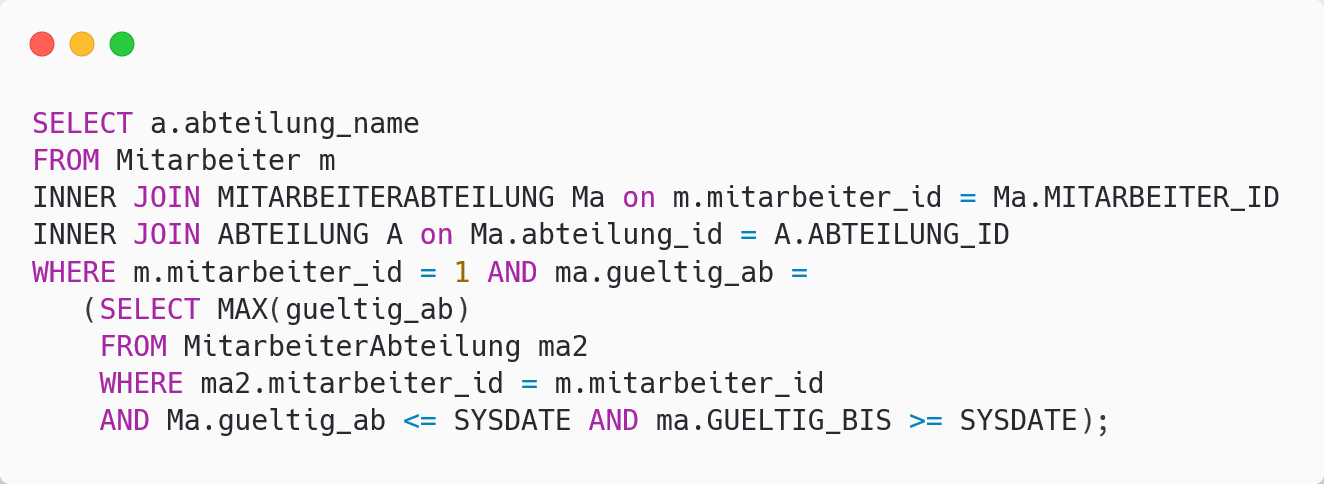
\includegraphics[width=\textwidth]{res/themenkorb_4/history_n_m.png}
\end{figure}

\section{Supertyp/Subtyp}
\subsection{Wann?}
\begin{itemize}
    \item Wenn zwei Entities einige Attribute gemeinsame haben, sich aber auch in einigen unterscheiden
    \item Beispiel: Lehrer \& Schüler
    \begin{itemize}
        \item Beide haben Eigenschaften einer jeden \textbf{Person} (Vorname, Nachname)
        \item Schüler haben außerdem eine Klasse, Lehrer ein Kürzel!
    \end{itemize}
    \item Lösung: Es werden 3 Tabellen erstellt (Person, Schüler, Lehrer); der Primary Key in Schüler / Lehrer ist gleichzeitig ein Foreign Key auf die Person!
    \item Nur dann sinnvoll, wenn es eine endliche Anzahl an Subtypen gibt, sonst sind dynamische Eigenschaften (|Eine Entity hat Liste aus Eigenschaften, diese wiederrum einen Wert für eine konkrete Entity) sinnvoller!
\end{itemize}

\section{Reflexive Beziehungen}
\subsection{Hierarchie}
\begin{itemize}
    \item Monohierarchie $\implies$ ein Parent
    \item (Polyhierarchie $\implies$ ggf. mehrere Parents)
\end{itemize}
\subsubsection{Varianten}
\begin{itemize}
    \item Variante 1 und 2
    \begin{itemize}
        \item Alle Ebenen haben identische Attribute
        \item Tabelle enthält einen Foreign Key auf sich selbst
        \item Je nach Umständen (Was ist Regel, was ist Ausnahme?) kann dieser Foreign Key optional (Variante 1) oder required (Variante 2) sein
    \end{itemize}
    \begin{figure}[H]
        \centering 
        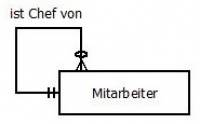
\includegraphics{res/themenkorb_4/hierarchie_variante_2.jpg}
    \end{figure}
    \item Variante 3
    \begin{itemize}
        \item Die Ebenen haben verschiedene Attribute $\implies$ Extra Table für jede Stufe, welcher einen Foreign Key auf den Parent beinhaltet
        \item Problem: Anzahl an Ebenen ist fix vorgegeben
    \end{itemize}
    \item Variante 4
    \begin{itemize}
        \item Die Ebenen haben teilweise verschiedene Attribute $\implies$ Extra Table für jede Stufe, welcher einen Foreign Key auf den Parent beinhaltet + Supertyp für die gemeinsamen Attribute
        \item Problem: Anzahl an Ebenen ist fix vorgegeben
    \end{itemize}
    \begin{figure}[H]
        \centering 
        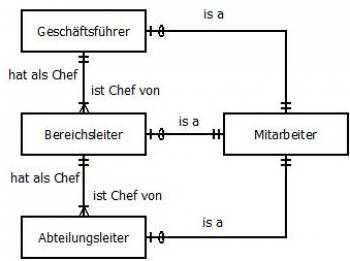
\includegraphics[scale=.8]{res/themenkorb_4/hierarchie_variante_4.jpg}
    \end{figure}
\end{itemize}
\subsection{Liste}
\begin{itemize}
    \item Gleich wie eine Hierarchie, nur dass der Foreign Key \textbf{unique} ist (auf eine Task kann nur eine folgen bzw. kann nur eine davor kommen!)
    \item Abfragen sind auch hier mittels hierarchischem SQL möglich!
\end{itemize}

\subsection{Gerichteter Graph (Netzplan)}
\begin{itemize}
    \item Eine Ausgangsentity (z.B. Stadt) + einen Verbindungstable (von, nach) mit 2 Foreign Keys auf Ausgangsentity
    \item Bidirektional --> View mithilfe von Union Erstellen, welcher von \& nach umdreht!
    \item Reflexive N:M Beziehung!
\end{itemize}

\section{Mehrwertige Beziehungen}
\begin{itemize}
    \item Wenn 3 fundamentale Entities in einem Satz vorkommen: Ein \textbf{Lehrer} unterrichtet eine \textbf{Klasse} in einem bestimmten \textbf{Fach}.
    \item Wenn viele N:M Beziehungen vorhanden sind
    \item Lösung: Eine verbindente Entity (z.B. Unterricht), welche mindestens 2 Foreign Keys im PK enthält
    \begin{itemize}
        \item Je nach Gestaltung des PKs können unterschiedliche Regeln festgelegt werden (Ein Lehrer darf eine Klasse nur in einem Fach unterrichten\dots)
    \end{itemize}
\end{itemize}